%!TEX program=xelatex

\documentclass[11pt]{ctexart}  
\usepackage[top=2cm, bottom=2cm, left=2cm, right=2cm]{geometry}  
\usepackage{algorithm}  
\usepackage{algorithmicx}  
\usepackage{algpseudocode}  
\usepackage{amsmath}  
\usepackage{graphicx}
\usepackage{amsmath}
\usepackage{amssymb}
\usepackage{enumerate}
\usepackage{booktabs}
\usepackage{fontspec}
\usepackage{listings}
\usepackage{xcolor}
\usepackage{paracol}

\newfontfamily\monaco{Monaco}
\definecolor{mygreen}{rgb}{0,0.6,0}
\definecolor{mygray}{rgb}{0.5,0.5,0.5}
\definecolor{mymauve}{rgb}{0.58,0,0.82}
\lstset{ %
backgroundcolor=\color{white},      % choose the background color
basicstyle=\footnotesize\ttfamily,  % size of fonts used for the code
columns=fullflexible,
tabsize=4,
breaklines=true,               % automatic line breaking only at whitespace
captionpos=b,                  % sets the caption-position to bottom
commentstyle=\color{mygreen},  % comment style
escapeinside=``,        % if you want to add LaTeX within your code
keywordstyle=\color{blue},     % keyword style
stringstyle=\color{mymauve}\ttfamily,  % string literal style
frame=single,
rulesepcolor=\color{red!20!green!20!blue!20},
language=python,
}

\floatname{algorithm}{算法}
\renewcommand{\algorithmicrequire}{\textbf{输入:}}  
\renewcommand{\algorithmicensure}{\textbf{输出:}} 

\title{密码学实验综合实验报告——基于SM2、SM3、SM4的安全文件传输协议}
\author{张天辰 17377321}

\makeatletter
\newenvironment{breakablealgorithm}
  {% \begin{breakablealgorithm}
   \begin{center}
     \refstepcounter{algorithm}% New algorithm
     \hrule height.8pt depth0pt \kern2pt% \@fs@pre for \@fs@ruled
     \renewcommand{\caption}[2][\relax]{% Make a new \caption
       {\raggedright\textbf{\ALG@name~\thealgorithm} ##2\par}%
       \ifx\relax##1\relax % #1 is \relax
         \addcontentsline{loa}{algorithm}{\protect\numberline{\thealgorithm}##2}%
       \else % #1 is not \relax
         \addcontentsline{loa}{algorithm}{\protect\numberline{\thealgorithm}##1}%
       \fi
       \kern2pt\hrule\kern2pt
     }
  }{% \end{breakablealgorithm}
     \kern2pt\hrule\relax% \@fs@post for \@fs@ruled
   \end{center}
  }
\makeatother

\begin{document}
\maketitle{}
\section{协议设计} % (fold)
\label{sec:协议设计}
\subsection{需求分析及框架} % (fold)
\label{sub:需求分析及框架}
本方案考虑双方传输文件的场景。在该场景下,双方的文件传输要求保密性、完整性与认证性。考虑到文件可能较大,为了兼顾效率,保密性可以用SM4算法提供;完整性和认证性可以由SM2数字签名提供。

考虑到并没有实质上可信的第三方来颁发数字证书,本算法并没有设置数字证书,发送方与接收方的公钥是公开发送的。考虑到有数字签名的存在,安全性能够得到保证。本方案使用带数字签名的Diffie-Hellman密钥交换协议交换对称加密密钥,保证密钥的安全。

本方案采用密文分组链接模式进行对称加密,则一共需要保密的内容有初始向量、文件名长度、文件名、明文消息及签名。初始向量可以用电码本模式加密,处于发送数据内容的最开始部分即可。
% subsection 需求分析及框架 (end)
\subsection{详细流程} % (fold)
\label{sub:详细流程}
\begin{enumerate}
    \item 双方首先建立连接,然后双方交换ID,再交换公钥。这一步类似于数字证书,只不过是没有可信第三方的签名。
    \item 在交换这些信息之后,双方就可以开始协商密钥。通过上一步的信息,可以验证数字签名,从而完成密钥的协商。
    \item 发送方发送文件长度和给接收方,这样接收方就可以判断接收多少长度的字节。此后,发送方产生初始向量,将这个值用上一步协商的密钥加密;将原始文件进行签名,拼接在文件后面,再使用对称密钥加密。将上述两个部分组合在一起,发送给接收方。
    \item 接收方得到发送的字节串,首先提取解密出初始向量,再用初始向量解密明文与签名,最后验证。只要验证通过,传输就结束了。
\end{enumerate}
% subsection 详细流程 (end)
% section 协议设计 (end)
\newpage{}
\newpage{}
\section{协议实现} % (fold)
\label{sec:协议实现}
本方案基于Python的socket套接字实现。
\begin{enumerate}
    \item 交换ID与公钥

    \begin{paracol}{2}
    \begin{lstlisting}[language={python},
    numbers=left,
    numberstyle=\tiny\monaco,
    basicstyle=\small\monaco]
    # sender
    socket.listen(5)
    sock, addr = socket.accept()
    socket.send(ID)
    targetID = socket.recv(10)
    # signature init
    auth = SM2Sign.SM2Sign(targetID) 
    socket.send(public)
    auth.public = sock.recv(65)
    \end{lstlisting}
    \switchcolumn
    \begin{lstlisting}[language={python},
    numbers=left,
    numberstyle=\tiny\monaco,
    basicstyle=\small\monaco]
    # receiver
    socket.connect((ip, port))
    senderID = socket.recv(10)
    # signature init
    auth = SM2Sign.SM2Sign(senderID) 
    socket.send(ID)
    auth.public = socket.recv(65))
    socket.send(public)
    \end{lstlisting}
    \end{paracol}
    \item 协商密钥

    发送方生成随机数$k_1$,然后发送$k_1 \cdot G$以及对其的签名;接收方同理生成$k_2$,发送$k_2 \cdot G$以及对其的签名。双方任意一方签名验证失败都会导致整个连接终止。如果双方都验签成功,则$K = k_1k_2 \cdot G$。协商成功。

    \begin{paracol}{2}
    \begin{lstlisting}[language={python},
    numbers=left,
    numberstyle=\tiny\monaco,
    basicstyle=\small\monaco]
    # sender
    sign = SM2Sign.SM2Sign(ID)
    sign.public = public
    sign.private = private
    k = randint(3, ECCPoint.n - 1)
    pt = point_to_bytes(SM2Sign.SM2Sign.g.multi(k))
    sig = sign.sign(pt)
    socket.send(pt || sig[0] || sig[1])
    other = socket.recv(130)
    otherPt = bytes_to_point(other[:65])
    otherSig = other[65:]
    if not auth.authenticate(other[:65], (otherSig[:32], otherSig[32:])):
        print("Authentication failed while key exchanging.")
        socket.close()
        sys.exit(0)
    key = point_to_bytes(otherPt.multi(k))[1:]
    \end{lstlisting}
    \switchcolumn
    \begin{lstlisting}[language={python},
    numbers=left,
    numberstyle=\tiny\monaco,
    basicstyle=\small\monaco]
    # receiver
    other = socket.recv(130)
    k = randint(3, ECCPoint.n - 1)
    otherPt = bytes_to_point(other[:65])
    otherSig = other[65:]
    if not auth.authenticate(other[:65], (otherSig[:32], otherSig[32:])):
        print("Authentication failed while key exchanging.")
        socket.close()
        sys.exit(0)
    key = point_to_bytes(otherPt.multi(k))[1:]
    sign = SM2Sign.SM2Sign(ID)
    sign.public = public
    sign.private = private
    pt = point_to_bytes(SM2Sign.SM2Sign.g.multi(k))
    sig = sign.sign(pt)
    socket.send(pt || sig[0] || sig[1])
    \end{lstlisting}
    \end{paracol}

    \item 消息发送

    在发送正式消息前,要先发送加密后消息长度。此后需要发送的消息格式如下:

    $E_{ecb}($初始向量$) || E_{cbc}($文件名长度 || 文件名 || 文件内容 || 签名$)$

    \begin{lstlisting}[language={python},
    numbers=left,
    numberstyle=\tiny\monaco,
    basicstyle=\small\monaco]
    # sender
    # signature init
    sign = SM2Sign.SM2Sign(ID)
    sign.public = public
    sign.private = private
    signature = sign.sign(src)

    encrypt = sm4.CryptSM4()
    encrypt.set_key(key, ENCRYPT)
    encryptIV = encrypt.crypt_ecb(iv)
    cipher = encrypt.crypt_cbc(
        iv, bytes([len(name)]) || name || src || signature)
    e = encryptIV || cipher
    # send the length first
    socket.send((len(e)).to_bytes())
    # send the rest
    for i in range(0, len(e), 1024):
        socket.send(e[i:i+1024])
    \end{lstlisting}

    \item 接收文件

    \begin{lstlisting}[language={python},
    numbers=left,
    numberstyle=\tiny\monaco,
    basicstyle=\small\monaco]
    # receiver
    length = socket.recv(3).to_int()
    l = 0
    target = b''
    while l < length:
        t = self.sock.recv(1024)
        target = b''.join([target, t])
        l += len(t)
    decrypt = sm4.CryptSM4()
    decrypt.set_key(self.key, DECRYPT)
    # the first 32 bytes are the encrypted iv
    iv = decrypt.crypt_ecb(target[:32])
    target = decrypt.crypt_cbc(self.iv, target[32:])
    nameLen = target[0]
    name = target[1:1+nameLen]
    result = auth.authenticate(target[1+nameLen:-64], (target[-64:-32], target[-32:]))
    if result:
        with open(name.decode(), "wb") as f:
            f.write(target[1+nameLen:-64])
        print("File received from " + sid)
    else:
        print("Authentication failed while receiving.")
        sys.exit(0)
    \end{lstlisting}
\end{enumerate}
% section 协议实现 (end)
\section{协议测试} % (fold)
\label{sec:协议测试}
在开始状态时,接收方文件夹只有代码文件,发送方文件夹除了代码文件外还有用于发送的文件(这个文件的位置可以是任意的),如图\ref{img_init}。

\begin{figure}[htbp]
\centering
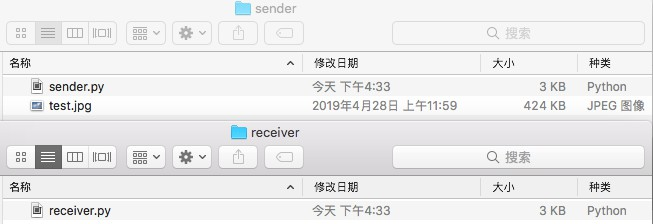
\includegraphics[width=13.06cm, height=4.48cm]{init.jpg}
\caption{初始状态}
\label{img_init}
\end{figure}

发送文件时的状态如图\ref{img_send}。

\begin{figure}[htbp]
\centering
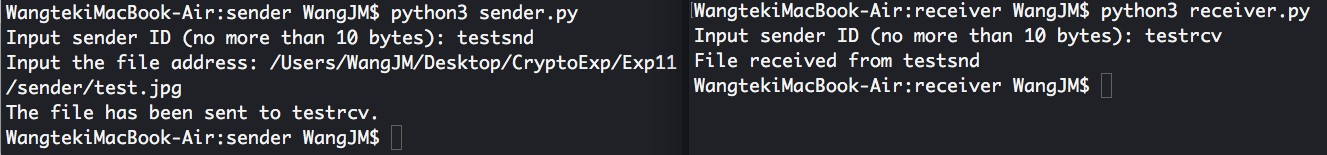
\includegraphics[width=13.27cm, height=1.55cm]{process.jpg}
\caption{发送文件}
\label{img_send}
\end{figure}

发送结束且接收结束后,接收方文件夹就出现了新的文件,其与发送方文件完全相同,如图\ref{img_rcv}。

\begin{figure}[htbp]
\centering
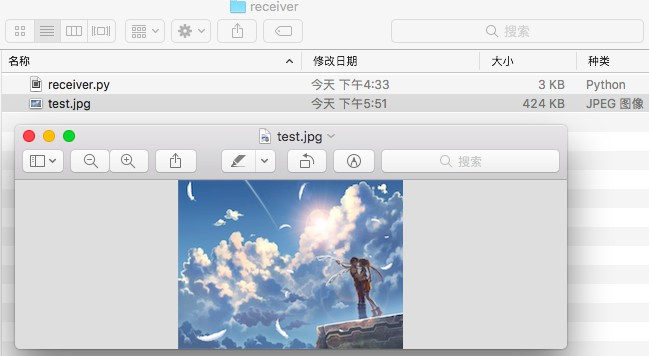
\includegraphics[width=12.98cm, height=6.12cm]{receive.jpg}
\caption{结束状态}
\label{img_rcv}
\end{figure}

接收方收到了jpg文件可以打开,说明解密完全正确,且数字签名验证成功。综上所述,根据测试结果,本方案的协议可以很好地工作。
% section 协议测试 (end)
\end{document}